
% ====================================================================
\chapter{Sorted Sequences}

Jeden Tag produziert die Menschheit ungefährt 2,5 Trillionen Bytes Daten, das sind ungefähr 1,7 Megabyte pro Person und pro Sekunde.\cite{techjury:20} Diese unglaublich großen Datenmengen werden gespeichert, verändert, aufgerufen und wieder gelöscht. Dabei spielen ausgreifte Datenstrukturen eine entscheidende Rolle, damit schnell und flexibel Daten bearbeitet werden können. Bei der Entwicklung von Datenstrukturen erkannte man sehr zeitig, dass es einfacher ist, eine geordenete Ansammlung von Daten zu verwalten, als eine zufällige Anordnung derer. Lange bevor das Internet oder Computer überhaupt existierten, wandte man dies bei Wörterbüchern und Lexika an. Wenn wir etwas nachschlagen wollen, finden wir es dort viel schneller, weil wir uns sicher sein können, das "`foo"' nach "`bar"' im Wörterbuch stehen muss.
\par
Sortierte Sequenzen funktionieren nach dem gleichen Prinzip. Wie in \autoref{fig:NavStruct} zu sehen, besteht eine sortierte Sequenz aus zwei Teilen. Einer geordneten, doppelt verketteten Liste, in der die Elemente anhand ihrer Schlüssel sortiert sind. Das würde schon ausreichen, aber man verwendet zusätzlich noch eine Navigationsstruktur, welche das Auffinden von Elementen deutlich beschleunigt. In einer doppelt verketteten Liste würde das Lokalisieren von einem Element $e_n$ bis zu $n$ Schritte benötigen, also müssen im schlimmsten Fall alle Elemente der Liste durchlaufen werden, um das gesuchte Element zu finden. \footnote{Man schreibt auch: $\mathcal{O} (n)$} Im Gegensatz dazu hat eine sortierte Sequenz mit einem (a,b)-Baum als Navigationsstruktur (Vgl. \autoref{section:ab-trees}) drastisch verbesserte Laufzeiten von bis zu $\log n$. \footnote{$\mathcal{O} (\log n)$} \cite{Sanders:19}
\par
Vergleicht man sortierte Sequenzen mit anderen Datenstrukturen, kann man sowohl Nach- als auch Vorteile feststellen. Einerseits ist der Aufbau einer sortierten Sequenz komplizierter als der einfachererer Datenstrukturen wie Feldern, sie sind allerdings deutlich flexibler, da sie das Einfügen und Entfernen von Elementen effizient unterstützen. Im Vergleich zu Hashtabellen sind sie langsamer, aber mächtiger, da man auch Elemente findet, wenn man nach einem Schlüssel $s$ sucht, zu dem kein Element $e$ existiert (genauer: man findet das Element $e'$ für das gilt: $s'\leq s$).
\par
Somit können sortierte Sequenzen die Anforderungen Geschwindigkeit und Flexibilität sehr gut erfüllen. Auf der Grundlage des Buches \textit{"`Sequential and Parallel Algorithms and Data Structures - The Basic Toolbox"'} \cite{Sanders:19} werde ich die Funktionsweise von sortierten Sequenzen erklären, wie sie in Kapitel 7 des genannten Buches beschrieben werden. Das Hauptaugenmerk wird auf sortierten Sequenzen mit (a,b)-Bäumen als Navigationsstruktur liegen, es sind jedoch auch diverse andere Arten von sortierten Sequenzen vorstellbar, welche auch in logarithmischer Zeit arbeiten können.

\begin{figure}
    \begin{center}
        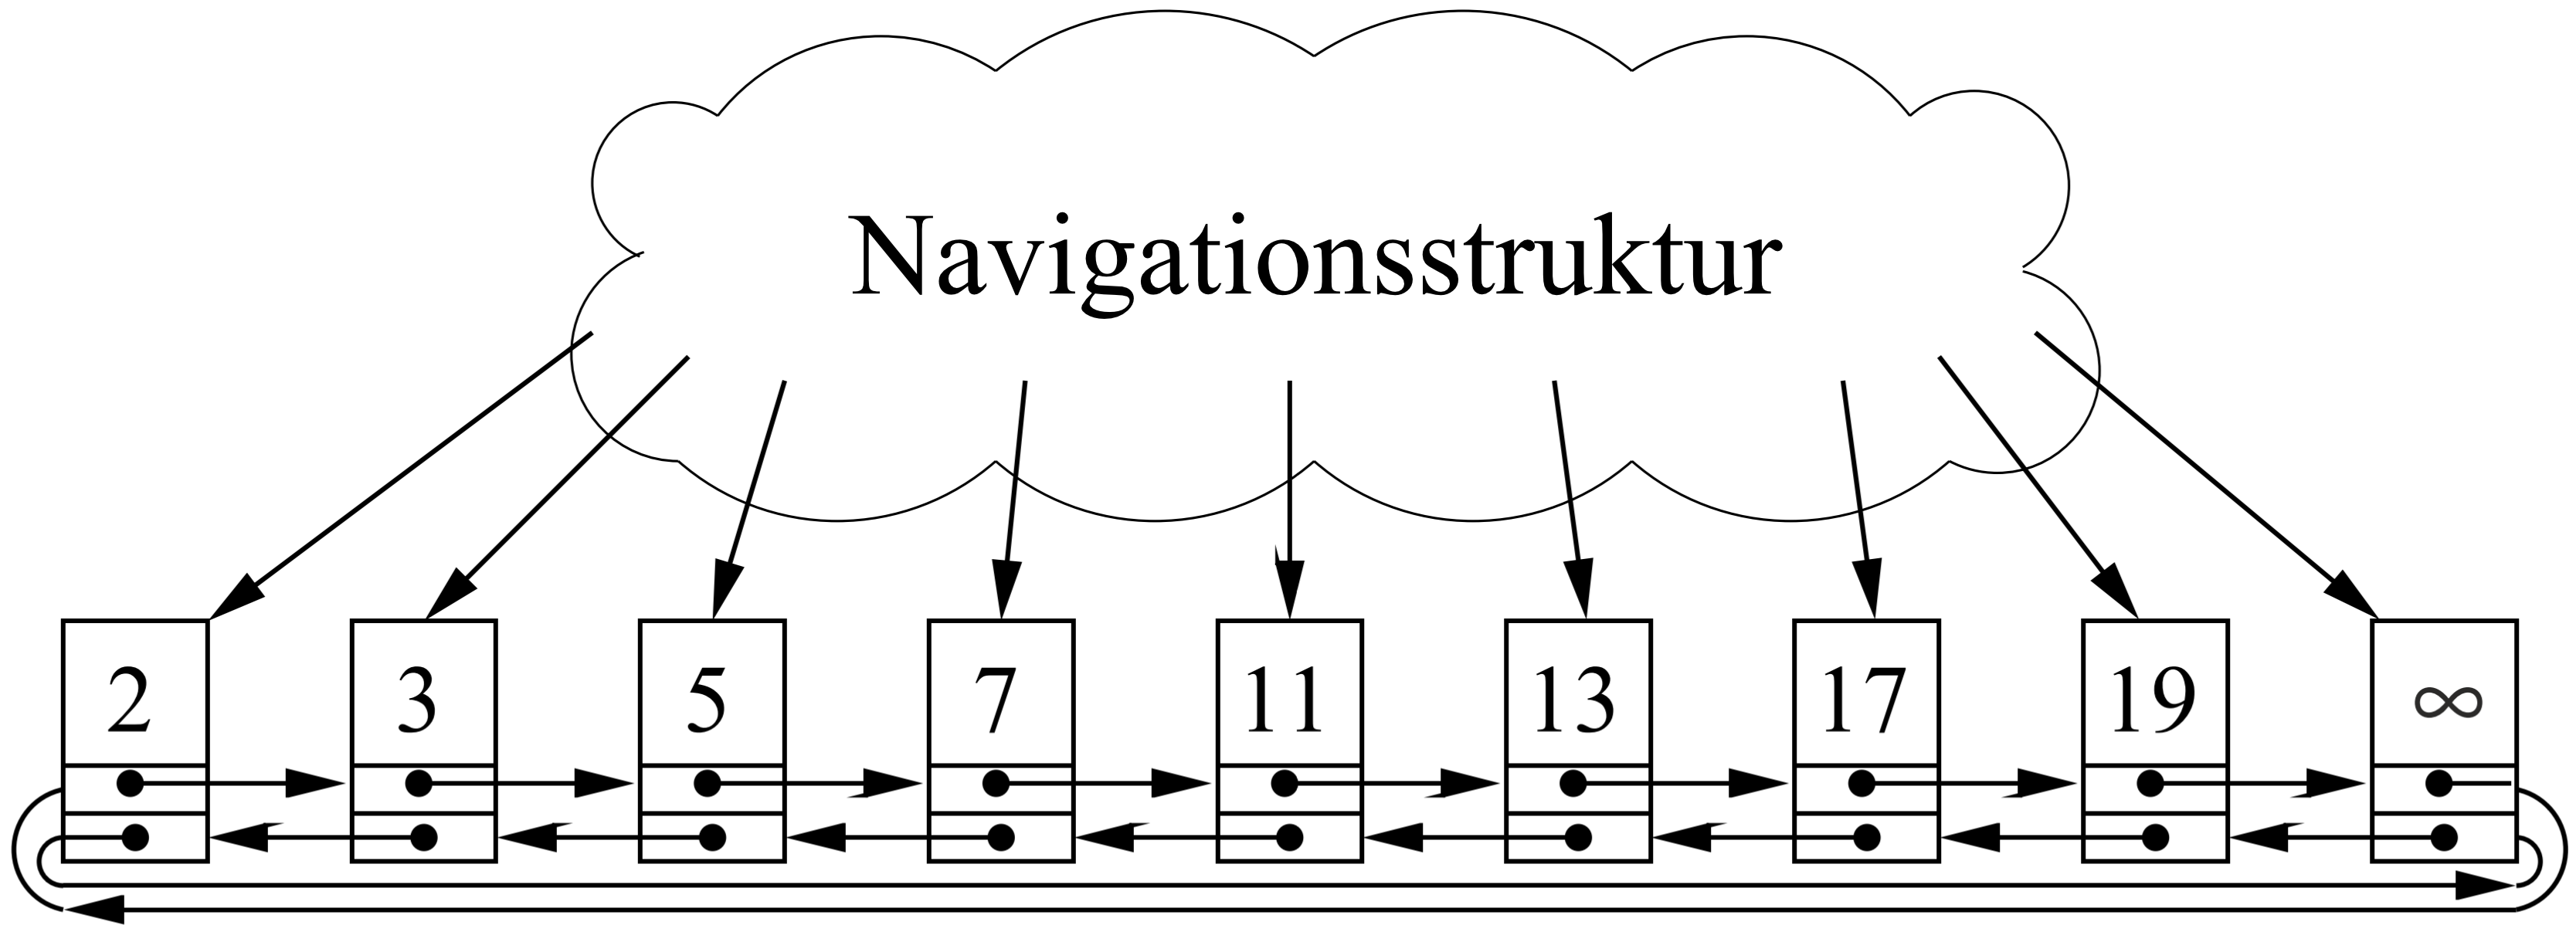
\includegraphics[width=0.8\linewidth]{assets/NavStruct.png}
        \caption{Eine sortierte Sequenz $\langle2, 3, \dots, 17, 19, \infty \rangle$, bestehend aus einer doppelt verketteten Liste und einer Navigationsstruktur. Das Dummy Element besitzt den Schlüssel $\infty$.\\\cite{Sanders:19}}
        \label{fig:NavStruct}
    \end{center}
\end{figure}


%--------------------------------------------------------------------
\section{Doppelt verkettete Listen}
\label{section:dll}

Verkettete Listen bestehen aus Elementen, die miteinander verknüpft werden. In einer einfach verketten Liste, zeigt jedes Element auf seinen Nachfolger, in einer doppelt verketteten Liste zeigt es zusätzlich auf seinen Vorgänger. Diese Struktur ermöglicht es, auf jedes Element zuzugreifen, auch wenn man anfangs nur ein Element gegeben hat. Des Weiteren sind vielseiteige Modifizierungen umsetzbar, namentlich das Einfügen und Löschen von Elementen oder von Teillisten, sowie das Verknüpfen von Listen. Ein Direktzugriff wird nicht unterstützt, da zuerst durch die Liste iteriert werden muss, um auf ein Element zuzugreifen.
\par
Einfach verlinkte Listen benötigen weniger Platz und sind schneller als doppelt verkettete Listen, weshalb es meistens besser ist, einfach verkettete Listen einzusetzen, wenn ihre Funktionalität ausreichend ist. Für sortierte Sequenzen benötigen wir jedoch doppelt verkettete Listen. \cite{Sanders:19}
\par
Die Anforderungen an eine doppelt verkettete Liste sind relativ simpel und führen bei Einhaltung zur korrekten Funktionsweise. Für jedes Element sollte $e_n$ gelten, dass der Vorgänger des Nachfolgers $e_{n+1}$ wieder das Element $e_n$ ist, und dass der Nachfolger des Vorgängers $e_{n-1}$ auch das Element $e_n$ ist. Somit können die Operationen $next$ und $previous$ ausgeführt werden, um durch eine doppelt verkettete Liste zu iterieren.\cite{Sanders:19}
\par
Doppelt verkettete Listen sind in sortierten Sequenzen für das Speichern der Daten zuständig, während die Navigationsdatenstruktur für das Lokalisieren derselben eingesetzt wird. In \autoref{fig:NavStruct} ist dies dargestellt. Zu beachten ist, dass das sogenannte "`Dummy Element"'\footnote{In \autoref{fig:NavStruct} besitzt es den Schlüssel $\infty$} kein Element im engen Sinne ist, da es ausschließlich die Pointer zu Nachfolger und Vorgänger enthält, jedoch keinen Wert. Dieses Dummy Element ist jedoch von entscheidender Bedeutung, da es so lange besteht, wie die Liste selbst besteht und somit immer den Zugriff auf alle restlichen Elemente gewährt. Diesen Weg habe ich auch in meiner Implementierung gewählt, worauf ich im Detail in \autoref{chapter:implementierung} eingehen werde.


%--------------------------------------------------------------------
\section{Binäre Suchbäume}
\label{section:binary-trees}

Eine sortierte Sequenz benötigt eine Navigationsstruktur, die das Auffinden von Elementen beschleunigt. Eine Möglichkeit kann sein, binäre Suchbäume zu benutzen. Dessen Funktionweise werden wir nun betrachten.
\par
Wer das Konzept der binäre Suche verstanden hat, kann dieses einfach auf binäre Suchbäume anwenden. Bei der binären Suche wird das "`Teile und Herrsche"'-Prinzip angewandt, man teilt den Datensatz, und vergleicht den Suchschlüssel mit der Stelle, an der man geteilt hat. Ist der Schlüssel kleiner oder gleich dem größten Element im linken Datensatz \footnote{bei Sortierung von klein nach groß, beziehungsweise von links nach rechts} wird die Suche auf den linken Datensatz beschränkt und wieder geteilt. Diese Vorgehensweise wird so oft wiederholt, bis nur noch ein Element übrig bleibt. Dieses Element muss dann den Schlüssel besitzen, wenn es im Datensatz vorhanden war.
\par
Ein binärer Suchbaum besteht aus "`Knotenpunkten"' und "`Blättern"'. Knoten speichern Schlüssel, welche den Weg zum gesuchten Element weisen. Diese Teiler-Schlüssel geben den maximalen Wert der Blätter in dem Unterbaum an, welcher sich auf der Linken Seite des Knotenpunktes befindet. Für alle Blätter im linken Unterbaum des Knotenpunktes mit dem Teilerschlüssel $s_t$ gilt $s \leq s_t$.
\par
Um ein Element mit dem Schlüssel $s$ zu finden, gilt also folgende Vorgehensweise: Man startet an der Wurzel des Baumes, sprich der Knotenpunkt ohne Eltern, der in einer visuellen Darstellung ganz oben stehen würde. Ist der Suchschlüssel $s_s$ kleiner oder gleich dem Teilerschlüssel $s_t$, steigt man in den linken Unterbaum ab. Ist $s_s>s_t$, führt man das Verfahren im rechten Unterbaum weiter. Falls das Element $e$ mit dem Schlüssel $s=s_s$ exisitiert,wird man es so finden. Falls das nicht der Fall sein sollte, gibt es zwei Möglichkeiten. Entweder der Unterbaum enthält den Vorgänger des Elementes gesuchten Elementes, $e'$ oder das gesuchte Element wäre der Nachfolger von $e'$. Ersteres tritt auf, wenn $s_s \leq Schlüssel(e')$ und zweiteres ist anzunehmen, wenn $s_s>Schlüssel(e')$. \cite{Sanders:19} Die doppelt verkettete Liste erledigt dann den Rest.
\par
Die Anzahl der Ebenen von der Wurzel bis zu den Blättern bezeichnet man als \textit{Höhe} des Suchbaumes. Bei Bäumen mit $n+1$ Blättern und einer Höhe von $\lceil \log (n+1) \rceil$ bezeichnet man als perfekt ausbalanciert.\footnote{$n$ Elmente und ein Dummy Element, daher $n+1$} Da an bei der Suche an jedem Knotenpunkt ein Schritt benötigt wird, entspricht die Zeit für das Suchen der Höhe des Baumes, das heißt $\mathcal{O}(\lceil \log (n+1) \rceil)$.\cite{Sanders:19} Dieser Wert ist sehr anstrebenswert, da er eine deutliche Verbesserung gegenüber anderen Datenstrukturen bietet, wie zum Beispiel die Doppelt verkettete Liste alleine. Wenn wir es mit einem gleichbleiben Datensatz zu tun hätten, wäre das ohne Abstriche zu genießen. Das entspricht aber leider nicht der Realität. Beim Einfügen und Entfernen von Elementen müsste der Baum balanciert bleiben, das Ausgleichen benötigt allerding viele Resourcen. Beim unkontrollierten Einfügen könnte es im schlimmsten Fall passieren, dass jeder Knotenpunkt auf der einen Seite zu einem Blatt zeigt und auf der anderen Seite zu dem restlichen Unterbaum. An diesem Punkt ist der Baum nicht besser als eine Liste.
\par
Da beim zufälligen Einfügen von Elementen nicht immer der schlimmste Fall eintritt, kann man davon ausgehen, dass die Höhe zu $\approx 2,99 \log n$ konvergiert. \cite{Sanders:19}


%--------------------------------------------------------------------
\section{(a,b)-Bäume}
\label{section:ab-trees}

Wie in \autoref{section:binary-trees} erwähnt, ist es sehr aufwendig, binäre Suchbäume zu balancieren. Bei jeder Operation \footnote{Einfügen und Entfernen von Elementen} müsste der Baum zu einem großen Grad umstrukturiert werden. An diesem Punkt setzen \textit{(a,b)-Bäume} an. Sie agieren nach dem gleichen Prinzip, besitzen eine Wurzel und Knotenpunkte, die zu den Blättern führen. Der Unterschied liegt in den Knotenpunkten. Anstatt von zwei Verzweigungen hat jeder Knotenpunkt zwischen $a \in \mathds{N}$ und $b \in \mathds{N}$ Unterbäume. Man bezeichnet die Anzahl der Unterbäume, die von einem Knotenpunkt ausgehen, als Grad $d$ des Knotenpunktes. Für (a,b)-Bäume gilt: $a \leq d \leq b$, wobei eine leere Sequenz eine Ausnahmen bilden kann, da diese nur aus der Wurzel mit einem Kind, dem Dummy-Element besteht.  Des Weiterein definiert man $a \geq 2$ und $b \geq 2 a - 1$, da somit $d$ flexibel genug ist, um sicherzustellen, dass alle Blätter die gleiche Tiefe haben. Die Wichtigkeit dieser Anforderung an $a$ und $b$ werden wir in \autoref{section:insert-remove} erkennen. In der Literatur \cite{Sanders:19} werde $a$ und $b$ meistens als $2$ und $4$ definiert, da diese Werte einfacher zu visualisieren sind und man somit das Konzept schneller versteht. In \autoref{fig:24Tree} ist ein solcher (2,4)-Baum dargestellt.
\par
Jeder Knotenpunkt besteht aus einem Feld von Zeigern zu den Unterbäumen (Blätter oder weitere Knotenpunkte) $c[1\dots d]$, einem Feld von Zeigern zu Teilerschlüsseln $s[1 \dots d-1]$ und dem Grad $d$, um zu uberprüfen, ob die Invariante $a \leq d \leq b$ erfüllt wird, oder ob Knotenpunkten geteilt oder zusammengeführt werden müssen.
\\
Man betrachte einen Knotenpunkt mit $s[1 \dots d-1]$ und $c[1 \dots d]$. Für alle Blätter mit Schlüssel $k$ am Fuße des Unterbaumes $c[i]$ gilt: $s[i-1] < k \leq s[i]$. Diese Invariante ermöglicht die Suche in (a,b)-Bäumen, welche in \autoref{section:locate} genauer betrachtet wird. Bei Betrachtung von \autoref{fig:24Tree}, erklärt sich auch, wieso nur $d-1$ Teilerschlüssel vorhanden sind, und nicht $d$. Alle Elemente, die einen Schlüssel haben, der größer als der Teilerschlüssel $s[d-1]$ ist, müssen zwangsläufig zu $c[d]$ gehören. Zur Vereinfachung definiert man $s[d]$ als $\infty$, da jeder verbleibende Schlüssel die Anforderung $k \leq \infty$ erfüllt. Mehr dazu in \autoref{chapter:implementierung}.
\par
Bevor in \autoref{chapter:operations} auf Operationen an sortierten Sequenzen mit (a,b)-Bäumen eingegangen wird, gilt es noch eine wichtige Beobachtung zu machen. Die Höhe eines (a,b)-Baumes beschreibt die Anzahl der Ebenen, beziehungsweise die maximale Anzahl von Knotenpunkten die man auf dem Weg von der Wurzel bis zu einem Blatt in einem gegebenen Baum maximal auffindet. Da man bei der Suche einen Baum von Wurzel bis zum gesuchten Blatt durchschreitet, ist die Höhe von entscheidender Bedeutung für die Laufzeit von Operationen. Für einen Baum mit $n$ Elementen beträgt die Höhe maximal $1+ \lfloor \log_{a}(n+1)/2 \rfloor$. \cite{Sanders:19}
\\
In diese Formel kann man beliebige Werte einsetzen und man merkt schnell, dass die Höhe bei steigender Anzahl von Elementen weiterhin klein bleibt. Diese Eigenschaft macht (a,b)-Bäume ideal für große Datenmengen, da schnelle Zugriffszeiten garantiert sind. In der vorliegenden Litartur liegt das Hauptaugenmerk auf (a,b)-Bäumen, und diesem Beispiel werde ich folgen.

\begin{figure}
    \begin{center}
        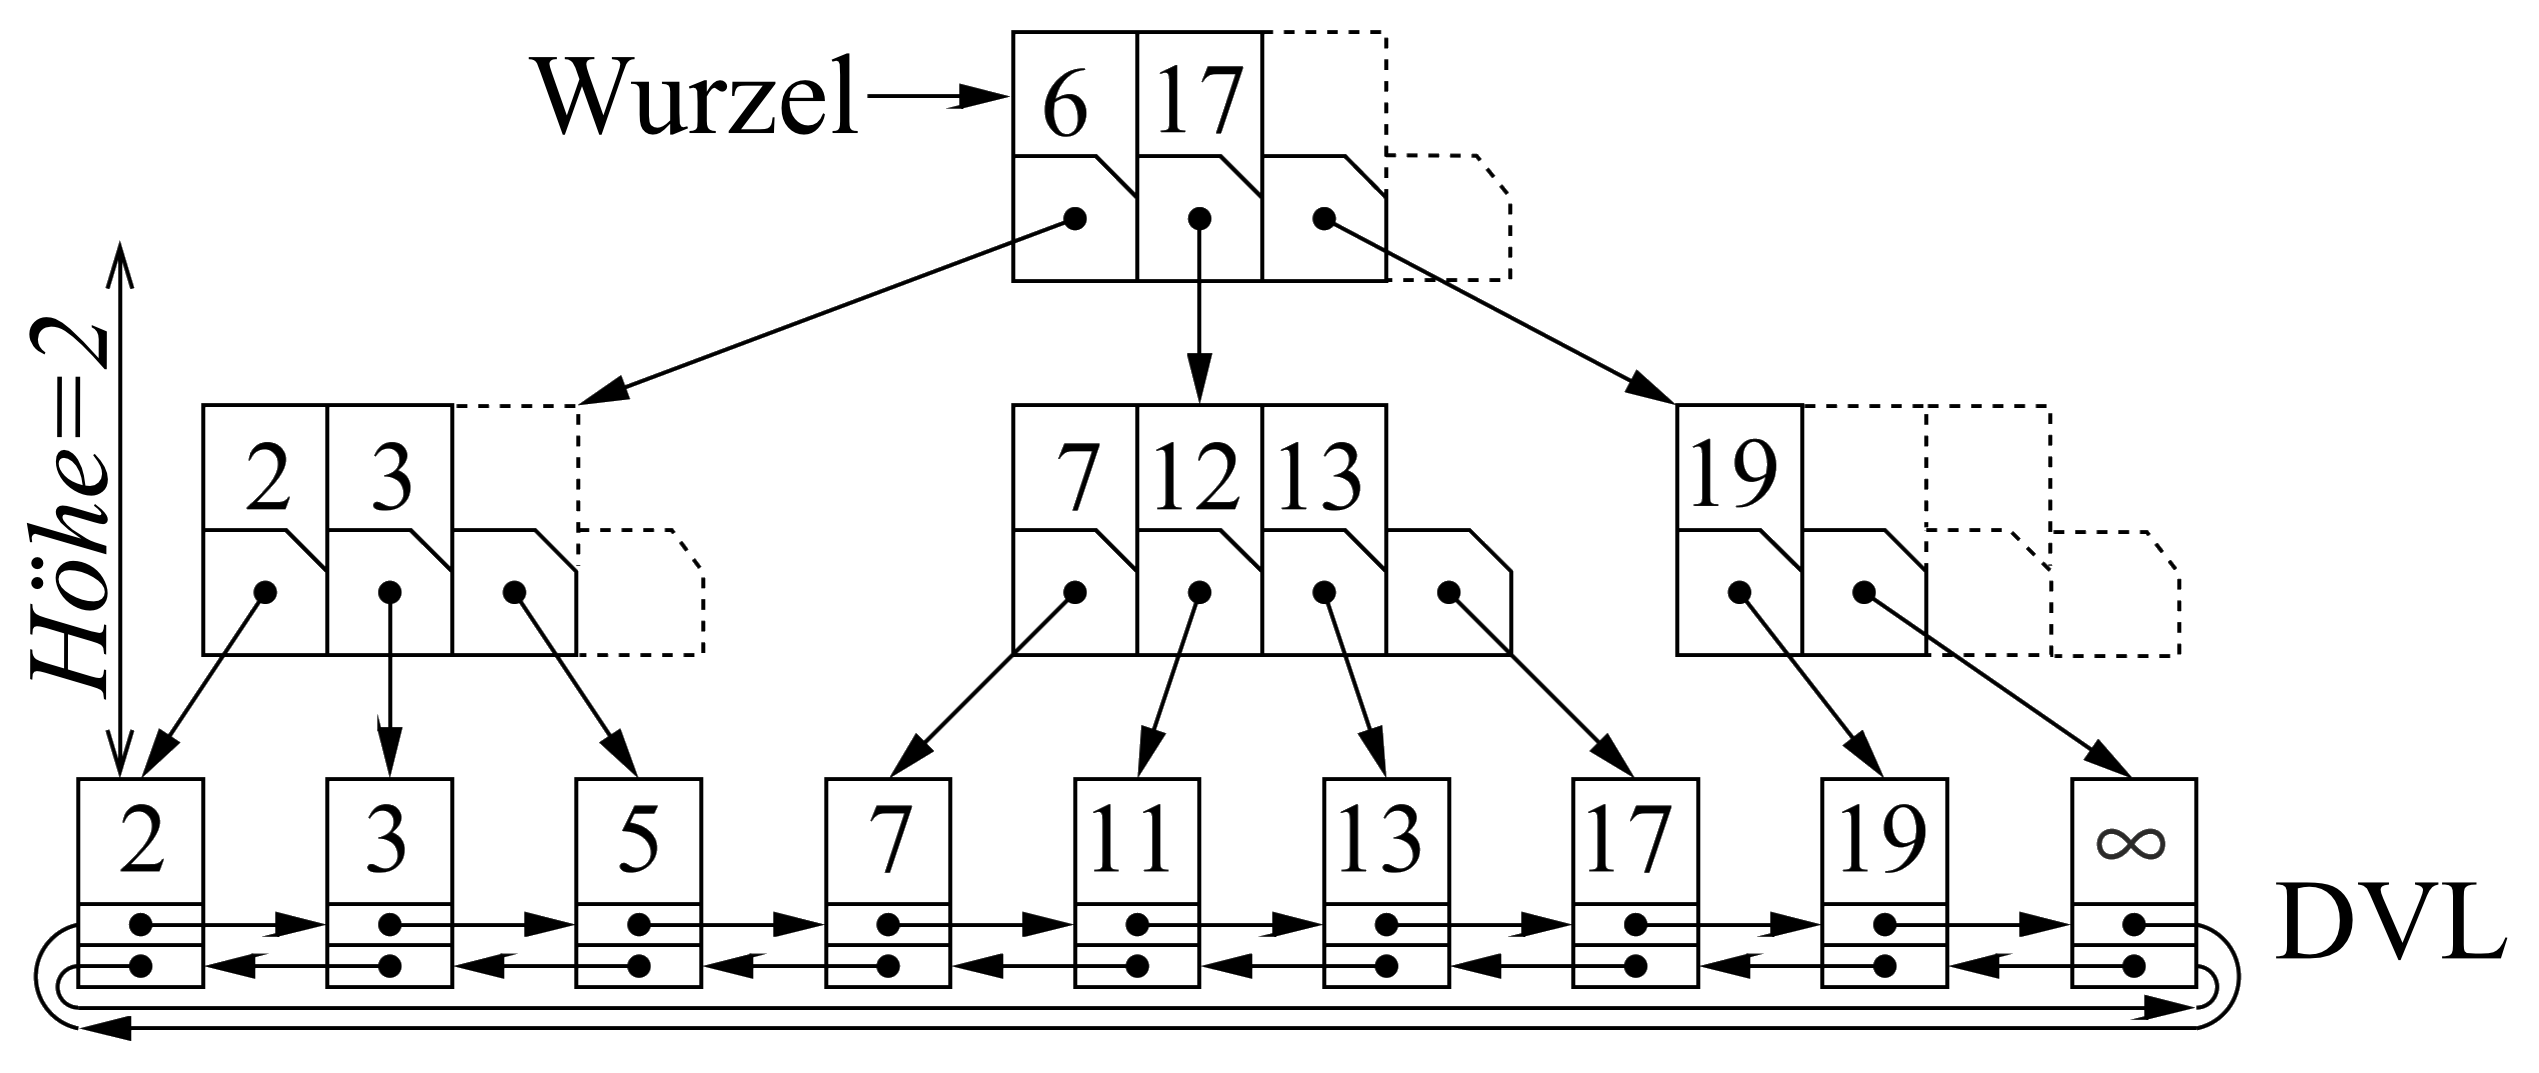
\includegraphics[width=0.8\linewidth]{assets/24tree.png}
        \caption{Ein (2,4)-Baum über einer doppelt verketteten List (DVL).\\\cite{Sanders:19}}
        \label{fig:24Tree}
    \end{center}
\end{figure}


% ====================================================================
\chapter{Operationen an Sortierten Sequenzen}
\label{chapter:operations}

In diesem Kapitel werde ich auf fünf verschiedene Operationen an sortierten Sequenzen eingehen. Die ersten drei, das \texttt{Finden}, \texttt{Einfügen} und \texttt{Entfernen} von Elementen werde ich ausführlicher behandeln, als das \texttt{Teilen} und \texttt{Zusammenführen} von ganzen Sequenzen, da sie ausführlicher dokumentiert sind und ich sie in Python implementiert habe. Nach den einzelnen Erläuterungen werde ich des Weiteren auf die Laufzeiten der Operationen eingehen.

%--------------------------------------------------------------------
\section{Finden}
\label{section:locate}

Um ein Element zu finden, muss man dem richtigen Pfad folgen, der einem zum gewünschten Element führt. Der Schlüssel $s_s$ stellt die Eingabe dar. Wie bei binären Suchbäumen startet die Suche an der Wurzel, aber ist etwas komplizierter. Anstatt von nur einem Vergleich an jedem Knotenpunkt, müssen mehrere Vergleiche getätigt werden, da ein Knotenpunkt mehr als zwei Verzweigungen haben kann. An jedem Knotenpunkt soll, das Kind $c[i]$ identifiziert werden, für das gilt: $s[i-1] < k < s[i]$, wobei $s[i]$ den zu $c[i]$ zugehörigen Teilerschlüssel darstellt, $s[i-1]$ den Teilerschlüssel des Kindes links von $c[i]$ und $k$ den Suchschlüssel. In anderen Worten vergleicht man $k$ mit den Teilerschlüsseln, bis man den kleinsten Teilerschlüssel findet, der größer oder gleich $k$ ist. Aufgrund des in \autoref{section:ab-trees} beschriebenenen Aufbau kann man sich sicher sein, dass sich das gesuchte Element mit dem Schlüssel $k$ im Unterbaum des Kindes $c[i]$ befindet, insofern es existiert. Der Vorgang wird bei $c[i]$ weitergeführt, bis man den Fuß des Baumes erreicht.
\par
Um zu wissen, wann der Fuß des Baumes erreicht ist, übergibt man am Anfang der Suche den Parameter $h$, der die Höhe des Baumes angibt. Jedes Mal, wenn man eine Ebene weiter absteigt, reduziert man $h$ um $1$. Sobald $h = 1$ erreicht ist, weiß man, dass die Kinder des aktuellen Knotenpunktes Blätter sind, also Elemente enthalten.
\par
Falls das Element mit Schlüssel $k$ im Baum enthalten ist, endet die Suche bei diesem Element und ist erfolgreich. Ist dies nicht der Fall, enthält der aktuellen Knotenpunkt \footnote{Der letzte Knotenpunkt in der Suche, wenn $h = 1$} das Element mit $k'$, wobei $k' > k$ ist oder den Vorgänger dieses Elements bei $c[d]$. Dann gibt man das Nachfolger-Blatt von $c[i]$ zurück, welches einen größeren Schlüssel als $k$ haben wird.
\par
\textbf{Laufzeit: } Wenn man für die Vergleiche an den Knotenpunkten binäre Suche verwendet, braucht man maximal $\lceil \log b \rceil$ Vergleiche pr Knotenpunkt. Die maximale Anzahl an Vergleichen pro Suche ist $\lceil \log b \rceil (1+\log_a((n+1)/2))$, da der zweite Teil dieses Terms die Höhe des Baumes beschreibt, und somit auch die Anzahl an Knotenpunkten angibt, die von der Suche durchlaufen werden müssen. Da sich die Anzahl der Vergleiche auf einen konstanten Durchschnittswert belaufen \footnote{Da $b$ konstant ist und somit die Anzahl immer $\leq \log b$ ist}, ist die Laufzeit für das \texttt{Finden} eines Elementes linear von der Größe des Baumes und somit logarithmisch von der Anzahl $n$ der Elemente abhängig.\\
\cite{Sanders:19}

%--------------------------------------------------------------------
\section{Einfügen \& Entfernen}
\label{section:insert-remove}

Um eine Element einzufügen oder zu entfernen, muss zuerst sein Platz gefunden werden, beziehungsweise das Element selbst. Dies wird rekursiv durchgeführt, da es so möglich ist, den Pfad wieder zurückzuverfolgen, nachdem das Element eingefügt oder gelöscht wurde. Das Finden wird wie in \autoref{section:locate} beschrieben durchgeführt. Im Folgenden nennen wir das einzufügenende Element $e$ mit dem Schlüssel $k$. Durch die Suche erhalten wir das Element $e'$ mit $k'$. Wenn $k = k'$, können wir das Element ersetzen und die Operation ist abgeschlossen, da jeder Schlüssel maximal ein Mal in der sortierten Sequenz vorkommt. Wenn $k < k'$ ist, muss das neue Element $e$ vor $e'$ in der doppelt verketteten Liste eingefügt werden. Kommen wir zum letzten Fall, wenn $k > k'$ ist. In diesem Fall wird logischerweise $e$ nach $e'$ eingefügt. In den beiden letzten Fällen müssen die Zeiger der Nachbarn von $e$ angepasst werden.
\par
Nun folgt der komplizierte Part, die Knotenpunkte über $e$ müssen gemäß der Invariante $a \leq d \leq$ angepasst werden, falls sie nicht erfüllt ist. Beim Einfügen von Elementen kann es passierem dass der Grad $d > a$ wird, und wieder reduziert werden muss. Dazu wird der betroffene Knotenpunkt in der Mitte geteilt. Das wird erreicht, indem man auf der linken Seite des Knotenpunktes einen neuen Knotenpunkt erschafft und die linke Hälfte der Kinder $c$ mit den dazugehörigen Teilerschlüsseln $s$ zu diesem neuen Knotenounkt verschiebt. Es ist darauf zu achten, die Werte von $d$ zu korrigieren und die Invariante $s[0] = - \infty, s[d] = \infty$ wiederherzustellen.
\\
Nun ist der Vorgang jedoch noch nicht abgeschlossen, da durch die Teilung der Grad der Eltern erhöht wurde. Da wir durch die Rekursion Zugriff auf die Elternknotenpunkte haben, können wir diesen Vorgehensweise so oft wiederholen, bis keine Teilung mehr nötig ist, oder wir bei der Wurzel angekommen haben, und diese notfalls auch geteilt haben. Beim Teilen der Wurzel muss eine neue Wurzel erstellt werden, und die Höhe des Baumes erhöht sich um eins.
\par
Beim Entfernen von Elementen kann es passieren, dass $d < a$ wird. Nun wird der betroffene Knotenpunkt $t$ mit seinem Nachbarn $u$ ausbalanciert. Es existieren zwei Fälle. Wenn $d$ von $u$ größer als $a$ ist, können eins oder mehrere Kinder von $u$ an $t$ übergeben. Wenn $d(u) = a$ ist, ist dies nicht möglich, da so $d(u) < a$ werden würde, und man das gleiche Problem wie anfangs hätte. Glücklicherweise kann man in diesem Fall $t$ und $u$ einfach miteinander kombinieren, und somit einen Knotenpunkt mit $d = 2a-1$ erschaffen. Dies kann die Invarianten des (a,b)-Baumes nicht verletzen, da die Anforderung $b \geq 2a-1$ existiert (Vgl. \autoref{section:ab-trees}).
\\
Wie beim Einfügen kann sich dieses Ausbalancieren bis zur Wurzel hocharbeiten und somit die Höhe des Baumes um eins verringern. Es gibt jedoch noch einen Sonderfall: Der Baum hatte bereits die Höhe 1, und besteht somit nur noch aus der Wurzel und dem Dummy Item. An diesem Punkt ist die Sequenz komplett geleert und die Höhe kann nicht weiter verringert werden.
\par
\textbf{Laufzeit: } Wie beim \texttt{Finden} sind die Laufzeiten von \texttt{Einfügen} und \texttt{Entfernen} linear abhängig von der Höhe des Baumes, und somit logarithmisch abhängig von der Anzahl der Elemente in der Sequenz.
\begin{quote}
    Für alle ganzen Zahlen $a$ und $b$ mit $a \geq 2$ und $b \geq 2 a - 1$, unterstützen (a,b)-Bäume die Operationen Einfügen, Löschen und Finden an sortierten Sequenzen der Größe $n$ in der Zeit $\mathcal{O}(\log n).$
        \hfill \cite{Sanders:19}
\end{quote}
Die hier beschriebene logarithmische Abhängigkeit der Laufzeiten von $n$ ist von entscheidender Bedeutigkeit für sortierte Sequenzen und deren Erfolg. Sie erreichen damit sehr kleine Zugriffszeiten, die bei wachsender Länge $n$ der Sequenz immer weniger schnell ansteigen. Somit haben sortiere Sequenzen einen großen Vorteil gegenüber anderen Datenstrukturen, deren Zugriffszeiten bei wachsendem $n$ schneller ansteigen.

%--------------------------------------------------------------------
\section{Teilen \& Zusammenfügen}
\label{section:split-merge}



%--------------------------------------------------------------------
\section{Amortisierte Analyse von Sorted Sequences}
\label{section:analyse}



%====================================================================
\chapter{Parallelisierung}
\label{chapter:Parallelisierung}



%====================================================================
\chapter{Implementierung in C}
\label{chapter:implementierung}
